\textbf{Answer: 5) $v_{\text{avg}} = 0$, $(v_{sp})_{\text{avg}} = 3\ \text{m/s}$, $a|_{t=6\ \text{s}} = 2\ \text{m/s}^2$}

\underline{\textbf{Solution for 5}}

$s = t^2 - 6t + 5$

$v = \dfrac{ds}{dt} = 2t - 6$

$a = \dfrac{dv}{dt} = 2$

$v = 0$ when $t = 3$

$\left.s\right|_{t=0} = 5$

$\left.s\right|_{t=3} = -4$

$\left.s\right|_{t=6} = 5$

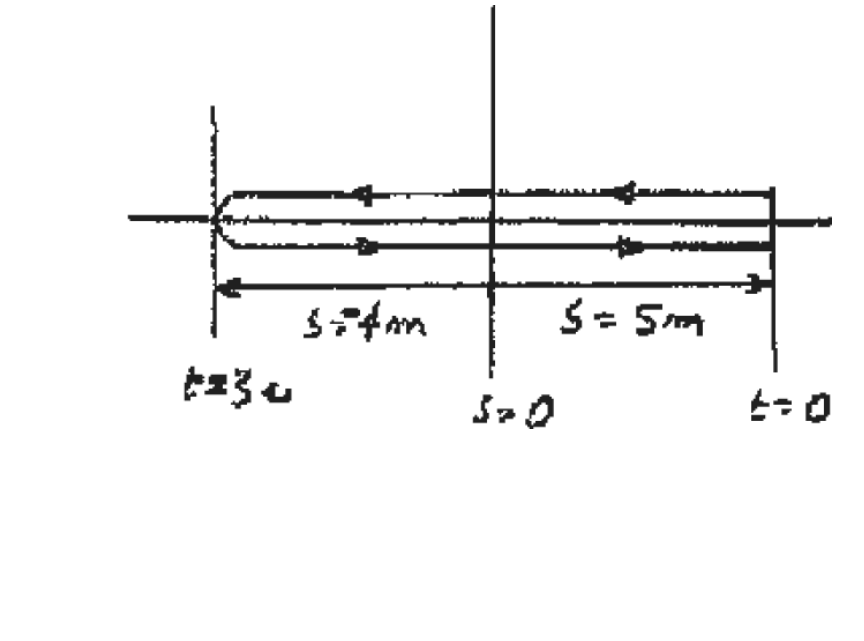
\includegraphics[width=\linewidth]{figures/sfig1.png}

$v_{\text{avg}} = \dfrac{\Delta s}{\Delta t} = \dfrac{0}{6} = 0$ \textbf{Ans.}

$(v_{sp})_{\text{avg}} = \dfrac{s_T}{\Delta t} = \dfrac{9 + 9}{6} = 3\ \text{m/s}$ \textbf{Ans.}

$a|_{t=6} = 2\ \text{m/s}^2$ \textbf{Ans.}